\documentclass[dvipsnames]{beamer}
\usepackage{polyglossia}
\usepackage{multicol}
\setdefaultlanguage{slovak}
\setbeamertemplate{caption}{\raggedright\insertcaption\par}
\setbeamerfont{caption}{size=\footnotesize}
\setbeamerfont{section in toc}{size=\small}
\setbeamerfont{subsection in toc}{size=\footnotesize}
\setbeamerfont{subsubsection in toc}{size=\scriptsize}
\setlength{\belowcaptionskip}{-13pt}
\setlength{\abovecaptionskip}{-5pt}
\setlength\intextsep{10cm}
\definecolor{bgc}{RGB}{250,250,250}
\definecolor{tc}{RGB}{0,0,50}
\definecolor{su}{RGB}{0,100,0}
\definecolor{g}{RGB}{0,210,10}
\urlstyle{same}
\setlength{\columnseprule}{0.1pt}
\setbeamercolor{sectionColor}{fg=white,bg=RoyalBlue}
\setbeamercolor{background canvas}{bg=bgc,fg=white}
\setbeamercolor{normal text}{fg=tc}
\setbeamercolor{frametitle}{fg=white,bg=ForestGreen}
\hypersetup{
	colorlinks=true,
	urlcolor={cyan},
	linkcolor=,
	pdfpagemode=FullScreen
}
\setbeamertemplate{section page}
{
	\begingroup
	\begin{beamercolorbox}[sep=12pt,center]{sectionColor}%
		\usebeamerfont{section title}\insertsection\par
	\end{beamercolorbox}
	\endgroup
}
\addtobeamertemplate{frametitle}{}{\vspace{-1.5em}}
\addtobeamertemplate{itemize subbody begin}{\scriptsize}

\begin{document}
\date{13. decembra 2023}
\title{Magnetická kvapalina - ferrofluid}
\author{Adam Jenča}
\begin{frame}
	\section{@TitlePage}
	\begin{center}
		\titlepage
	\end{center}
\end{frame}

\begin{frame}
	\section{Čo to je?}
	\frametitle{Čo to je?}
	\vskip .5cm
	\begin{itemize}
		\item Kvapalina priťahovaná k pólom magnetu
		\item Skladá sa z mikroskopicky malých magnetických častíc uložených v kvapaline (väčšinou olej)
		      \label{surfactantforgorurstupidbish}\item Každá častica je obalená v tenzide - látke schopnej znižovať povrchové napätie - aby sa zabránilo zrážaniu a pre lepšiu stabilizáciu častíc.

		\item Magnetické vlastnosti si mimo magnetického poľa neuchováva.
		\item Je to tzv. koloid - (mikroskopicky malé pevné častice v nejakej inej látke)
		\item
		      \href{https://turing.gjh.sk/~jenca.a/ferrofluid.mp4}{Video ferrofluidu v magnetickom poli}
	\end{itemize}
\end{frame}

\begin{frame}
	\section{História}
	\frametitle{História}
	\begin{itemize}
		\item Magnetická kvapalina bola vynájdená v roku 1963 Stevom Papellom v NASA.
		\item Pôvodne používaná v raketovom palive ktoré mohlo byť jednoducho presúvané v beztiažovom stave pomocou mag. poľa.
		\item V minulosti tiež využitá v lekárstve pri magnetickej rezonancii.
	\end{itemize}
	\begin{figure}
		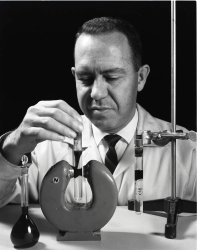
\includegraphics[scale=.45]{steve.png}
		\caption{Steve Papell}
	\end{figure}
\end{frame}
\begin{frame}
	\section{Zloženie}
	\frametitle{Zloženie}
	\begin{itemize}
		\item 5\% magnetická látka (magnetit / hematit)
		\item 10\% \hyperlink{surfactantforgorurstupidbish}{tenzid} (kyselina olejová, kyselina citrónová, sójový lecitín)
		\item 85\% olej / voda

	\end{itemize}
	\begin{figure}
		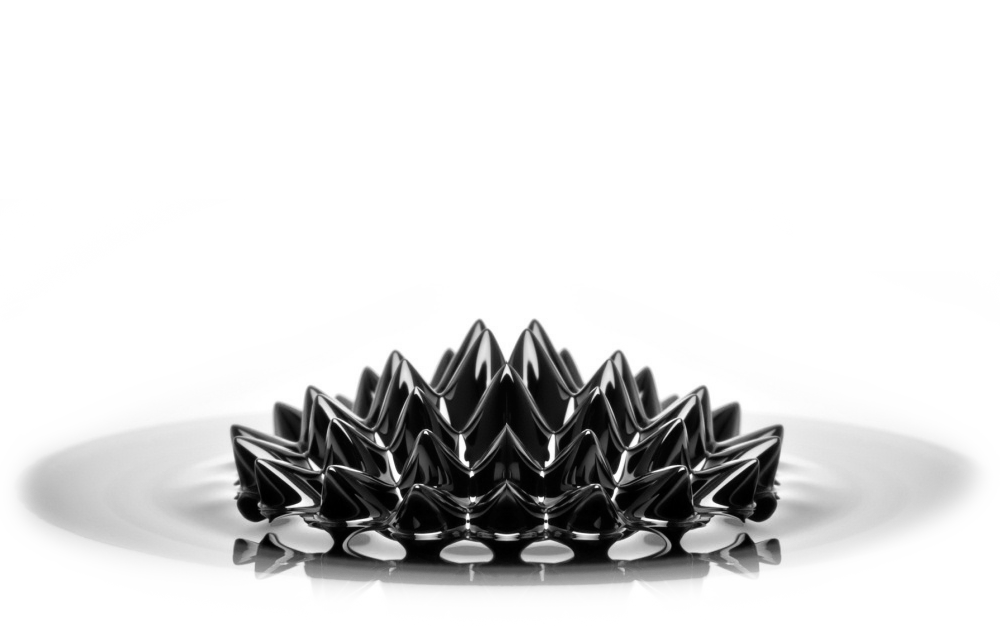
\includegraphics[scale=.2]{ferro2}
		\caption{Ferrofluid pod vplyvom mag. poľa}
	\end{figure}
\end{frame}
\begin{frame}
	\section{Využitie}
	\frametitle{Využitie}
	\begin{itemize}
		\item V elektronike na ochranu harddiskov pred nečistotami
		\item Ako mazadlo
		\item V reproduktoroch na ochladenie a mazanie cievok
		\item Triedenie buniek pri bunkovej terapii
		\item Vizualizácia hudby
		\item V umeleckých dielach(napr. sochách)
	\end{itemize}
	\begin{figure}
		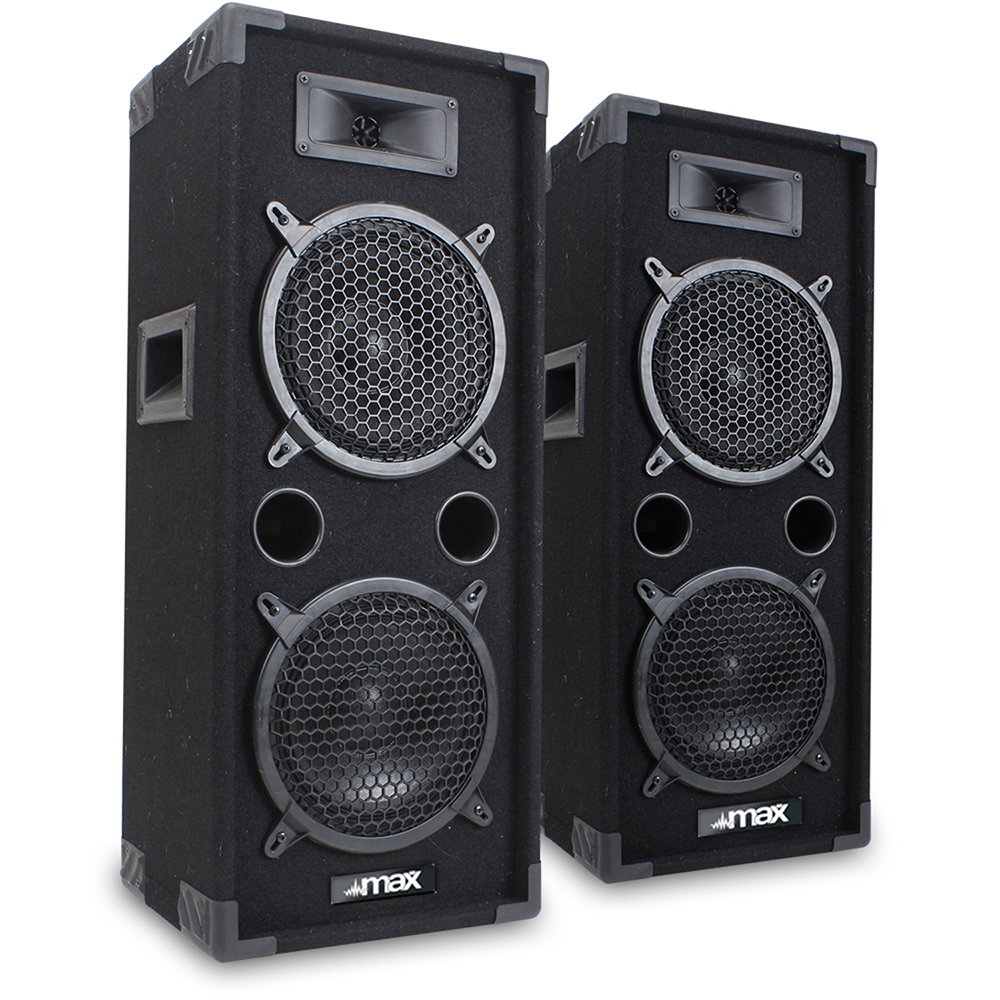
\includegraphics[scale=.1]{repr}
	\end{figure}
\end{frame}
\begin{frame}
	\section{Zdroje}
	\frametitle{Zdroje}
	{\tiny
		\begin{enumerate}
			\item \href{https://www.doi.org/10.1557/PROC-676-Y7.8}{Voit, W.; Kim, D. K.; Zapka, W.; Muhammed, M.; Rao, K. V. (21 March 2011). "Magnetic behavior of coated superparamagnetic iron oxide nanoparticles in ferrofluids". MRS Proceedings. 676.}
			\item \href{https://www.thoughtco.com/how-to-make-liquid-magnets-606319}{Helmenstine, Anne Marie. "How to Make Liquid Magnets". ThoughtCo.}
			\item \href{http://www.sbfisica.org.br/bjp/download/v25/v25a10.pdf}{Rlums, Elmars (1995). "New Applications of Heat and Mass Transfer Processes in Temperature Sensitive Magnetic Fluids". Brazilian Journal of Physics. 25 (2).}
			\item \href{https://www.czferro.com/ferrofluid-history}{"Brief History of Ferrofluid". Ferrofluid Displays, Art, and Sculptures | Concept Zero.}
		\end{enumerate}}
\end{frame}
\end{document}
